\chapter{एककोशिकीय जीवों की विविधता}\label{ch:b2:unicellular-diversity}

सूक्ष्मदर्शी के नीचे तालाब के पानी की एक बूँद में दो कशाभों से नाव खेती
एक हरी कोशिका है, जीवाणुओं को अपनी गुहिका में बुहारता एक चप्पल-आकार का
पक्ष्माभी है, पट्टी पर सरकता एक काचाभ डायटम है और, ठीक से दिखने में
बहुत छोटे, हज़ार जीवाणु हैं। हर एक अकेली कोशिका है और हर एक पूरा जीव है:
वह एक ही कोशिका के रूप में खाता, चलता, संवेदन करता, बढ़ता, जनन करता और
मरता है। सजीव जगत् का अधिकांश भाग सदा से ऐसा ही रहा है। यह अध्याय
\omterm{def:b2:unicellular-diversity:unicellular}{एककोशिकीय जीव} को एक अभिकल्प-समस्या की तरह लेता है --- एक कोशिका
क्या कर सकती है और क्या नहीं --- और प्राक्केंद्रकियों तथा सुकेंद्रकियों
के ढूँढ़े उत्तरों का सर्वेक्षण करता है, उस बिंदु तक जहाँ कोशिकाएँ साथ
रहने लगती हैं।

\section{एक कोशिका, सारे कार्य}

\begin{definition}[एककोशिकीय, निवही, बहुकोशिकीय]\label{def:b2:unicellular-diversity:unicellular}
कोई जीव \emph{एककोशिकीय}\index{एककोशिकीय जीव} तब है जब एक ही कोशिका
जीवन के हर कार्य को --- पोषण, विनिमय, गति, जनन --- निभाती है और अपने
भरोसे जीती है। वह \emph{निवही}\index{निवही जीव} तब है जब एक ही प्रकार
की कोशिकाएँ विभाजन के बाद जुड़ी रह जाती हैं पर अलग कर दी जाएँ तो हर एक
अकेली जी सकती है। वह \emph{बहुकोशिकीय}\index{बहुकोशिकीय जीव} तब है जब
उसकी कोशिकाएँ कई प्रकार की हैं, एक-दूसरे पर निर्भर हैं, और उनमें से
थोड़ी ही (जनन वंशक्रम) संतति छोड़ती हैं। एककोशिकीय जीवों में सारे
आर्किया, लगभग सारे जीवाणु और सुकेंद्रकियों के अधिकांश वंशक्रम आते हैं;
अनौपचारिक नाम \emph{\omterm{def:b2:unicellular-diversity:protist}{प्रोटिस्ट}} एककोशिकीय सुकेंद्रकियों को समेटता है,
जो एक समूह नहीं बल्कि अनेक हैं।
\end{definition}

\begin{example}[एक बूँद के छह निवासी]\label{ex:b2:unicellular-diversity:drop}
\emph{Escherichia coli}, \qty{2}{\micro m} लंबी एक छड़, कशाभों के गुच्छे
से तैरती है और भरपेट हो तो हर बीस मिनट में विभाजित होती है।
\emph{Chlamydomonas}, \qty{10}{\micro m} चौड़ी एक हरी शैवाल, दो कशाभों से
उस प्रकाश की ओर नाव खेती है जिसे वह नेत्रबिंदु से भाँपती है।
\emph{Paramecium}, \qty{200}{\micro m} का एक पक्ष्माभी, हज़ारों पक्ष्माभों
से ढका है, गुहिका से भोजन लेता है और दो संकुचनशील रसधानियों से पानी
उलीचता है। कोई डायटम सिलिका के दो-भागी कवच में रहता है, जो छिद्रों से
अलंकृत है। \emph{Amoeba} कूटपाद बढ़ाकर बहता है और जो मिले उसे निगल लेता
है। खमीर की कोशिका अपनी बगल से एक पुत्री-कोशिका का मुकुल निकालती है।
एक ही समस्या के छह उत्तर, बहुत भिन्न आकार और साज-सामान के।
\end{example}

\begin{omfigure}
\begin{tikzpicture}[x=1.9cm]
  % log scale from 0.1 um to 100 mm : position = log10(size in um) + 1
  \draw[thick] (0,0) -- (6,0);
  \foreach \p/\l in {0/{\qty{0.1}{\micro m}},1/{\qty{1}{\micro m}},2/{\qty{10}{\micro m}},3/{\qty{100}{\micro m}},4/{\qty{1}{mm}},5/{\qty{10}{mm}},6/{\qty{100}{mm}}}
    \draw (\p,0.12) -- (\p,-0.12) node[below, font=\scriptsize] {\l};
  \foreach \p/\c/\l in {0.5/omDef/माइकोप्लाज़्मा, 1.3/omDef/{\emph{E.~coli}}, 1.7/omDef/खमीर, 2.0/omProp/{\emph{Chlamydomonas}}, 2.7/omProp/डायटम, 3.3/omProp/{\emph{Paramecium}}, 3.65/omProp/{\emph{Amoeba proteus}}, 3.9/omThm/{\emph{Thiomargarita} (एक जीवाणु)}, 5.7/omProp/{\emph{Acetabularia}}}
    { \fill[\c] (\p,0) circle (0.05); \node[rotate=60, anchor=west, font=\scriptsize, \c, inner sep=1pt] at (\p,0.12) {\l}; }
  \node[font=\scriptsize, anchor=north] at (3,-0.55) {कोशिका का आकार (लघुगणकीय मापनी)};
\end{tikzpicture}

{\small \omterm{def:b2:unicellular-diversity:unicellular}{एककोशिकीय जीवों} के आकार परिमाण की पाँच कोटियों में फैले हैं।
\omterm{def:b2:unicellular-diversity:prokaryote}{प्राक्केंद्रकी} (नीले) एक माइक्रोमीटर के आसपास जमा हैं; सुकेंद्रकी
कोशिकाएँ (नारंगी) दस से सौ गुना बड़ी हैं; सबसे बड़ी अकेली कोशिकाएँ ---
कोई विशाल गंधक-जीवाणु, शैवाल \emph{Acetabularia} --- वे अपवाद हैं जिन्हें
पाठ समझाता है।}
\end{omfigure}

\begin{proposition}[पृष्ठ, आयतन और आकार की सीमा]\label{prop:b2:unicellular-diversity:surface}
\index{पृष्ठ-आयतन अनुपात}
कोई कोशिका अपने परिवेश से अपने पृष्ठ के रास्ते विनिमय करती है और अपने
आयतन के समानुपात में खपत करती है। $r$ त्रिज्या के किसी गोले के लिए
\emph{\omterm{prop:b2:unicellular-diversity:surface}{पृष्ठ-आयतन अनुपात}} है
\[
\frac{S}{V} = \frac{4\pi r^2}{\tfrac{4}{3}\pi r^3} = \frac{3}{r},
\]
यानी त्रिज्या दुगुनी करने पर कोशिकाद्रव्य की प्रति इकाई उपलब्ध पृष्ठ आधा
रह जाता है। इसलिए जो कोशिका अपने भीतरी भाग को खिलाने के लिए झिल्ली के आरपार
विसरण पर टिकी है वह अनिश्चित काल तक बढ़ नहीं सकती: किसी त्रिज्या पर पृष्ठ
से होती आपूर्ति आयतन की माँग पूरी करना छोड़ देती है। यही नियम बताता है कि
प्रति ग्राम सबसे अधिक उपापचयी सक्रियता छोटी कोशिकाओं में क्यों है, और बड़ी
कोशिकाएँ चपटी, लंबी, रसधानीदार या भीतरी झिल्लियों से भरी क्यों होती हैं।
\end{proposition}

\begin{theorem}[किसी दूरी को विसरण से पार करने का काल]\label{thm:b2:unicellular-diversity:diffusion}
\index{विसरण काल}
$D$ विसरण गुणांक वाला कोई अणु यादृच्छिक पगों में भटकता है; किसी काल $t$ के
बाद एक अक्ष पर उसका माध्य वर्ग विस्थापन
$\langle x^2\rangle = 2Dt$ होता है। इसलिए केवल विसरण से कोई दूरी $x$ तय
करने में लगने वाला काल है
\[
t \approx \frac{x^2}{2D},
\]
जो दूरी के \emph{वर्ग} के साथ बढ़ता है। जल में किसी छोटे अणु के लिए
$D \approx \qty{1e-9}{m^2/s}$ लेने पर, किसी जीवाणु (\qty{1}{\micro m}) को
पार करने में आधा मिलीसेकंड लगता है; \qty{1}{mm} की कोशिका को पार करने में
आठ मिनट लगते, और एक मीटर को पार करने में सोलह वर्ष।
\end{theorem}
\begin{proof}
मान लीजिए वह अणु $\ell$ लंबाई का एक पग हर $\tau$ सेकंड पर यादृच्छिक रूप
से बाएँ या दाएँ रखता है। $n$ पगों के बाद उसका विस्थापन
$x = \sum_i \varepsilon_i \ell$ है, जिसमें $\varepsilon_i = \pm 1$
स्वतंत्र हैं, इसलिए $\langle x\rangle = 0$ और $\langle x^2\rangle =
\sum_i \langle\varepsilon_i^2\rangle \ell^2 = n\ell^2$ (आड़े पद
औसत में शून्य हो जाते हैं)। $n = t/\tau$ रखने पर यह $\langle x^2\rangle
= (\ell^2/\tau)\,t$ है, और $D = \ell^2/2\tau$ लिखने पर
$\langle x^2\rangle = 2Dt$ मिलता है। $\langle x^2\rangle = x^2$ रखने पर
वह काल मिल जाता है।
\end{proof}

\begin{theorem}[किसी गोलीय कोशिका को विसरण से आपूर्ति]\label{thm:b2:unicellular-diversity:supply}
\index{विसरण-सीमित ग्रहण}
$r_0$ त्रिज्या की कोई गोलीय कोशिका, जो अपने पृष्ठ तक पहुँचने वाले किसी
विलेय के हर अणु को सोख लेती है, ऐसे माध्यम में जहाँ दूर की सांद्रता
$c_\infty$ है, स्थायी अवस्था में इतना अभिवाह (अणु प्रति सेकंड) पाती है:
\[
J = 4\pi D r_0\, c_\infty .
\]
आपूर्ति केवल $r_0$ के साथ बढ़ती है, जबकि माँग $r_0^3$ के साथ: किसी
त्रिज्या से आगे विसरण पर पलने वाली कोशिका भूखी रह जाती है।
\end{theorem}
\begin{proof}
स्थायी अवस्था में $r > r_0$ त्रिज्या के हर गोले को प्रति सेकंड पार करते
अणुओं की संख्या एक ही है, $J = 4\pi r^2 D\,
(\mathrm{d}c/\mathrm{d}r)$ (फ़िक का नियम, अभिवाह भीतर की ओर)।
इसलिए $r^2\,\mathrm{d}c/\mathrm{d}r = J/4\pi D$ अचर है; $r_0$ से, जहाँ
$c = 0$, अनंत तक, जहाँ $c = c_\infty$, समाकलन करने पर:
$c_\infty = (J/4\pi D)\int_{r_0}^{\infty} r^{-2}\,\mathrm{d}r =
J/(4\pi D r_0)$, जिससे $J = 4\pi D r_0 c_\infty$।
\end{proof}

\begin{example}[विसरण से पलने वाली कोशिका कितनी बड़ी हो सकती है?]\label{ex:b2:unicellular-diversity:howbig}
कोई वायुजीवी कोशिका प्रति घन मात्रा कोशिकाद्रव्य लगभग
$q = \qty{0.02}{mol/m^3/s}$ की दर से (एक तेज़ दर) ऑक्सीजन खपाती है। उसकी
माँग $q \cdot \tfrac{4}{3}\pi
r_0^3$ है; वायु-संतृप्त जल से आपूर्ति ($c_\infty =
\qty{0.25}{mol/m^3}$, $D = \qty{2e-9}{m^2/s}$) $4\pi D r_0
c_\infty$ है। बराबर रखने पर $r_0^2 = 3Dc_\infty/q = 3\times 2\times 10^{-9}
\times 0.25/0.02 = \qty{7.5e-8}{m^2}$, इसलिए $r_0 \approx
\qty{270}{\micro m}$। असल में सक्रिय कोशिकाएँ इससे कहीं नीचे रहती हैं,
क्योंकि ऑक्सीजन को उनके \emph{भीतर} भी विसरित होना पड़ता है;
\qty{750}{\micro m} का गंधक-जीवाणु \emph{Thiomargarita} इस सीमा से यों
बचता है कि वह लगभग पूरा का पूरा एक रसधानी है और उसका कोशिकाद्रव्य कुछ
माइक्रोमीटर गहरा एक पतला खोल भर है।
\end{example}

\begin{omfigure}
\begin{tikzpicture}
\begin{axis}[
  width=0.8\linewidth, height=6.2cm,
  axis x line=bottom, axis y line=left,
  xmode=log, ymode=log,
  xmin=0.3, xmax=1000, ymin=1e-6, ymax=1e4,
  xlabel={कोशिका की त्रिज्या (\unit{\micro m})}, ylabel={अणु प्रति सेकंड (सापेक्ष)},
  xlabel style={font=\small, at={(axis description cs:0.5,-0.1)}, anchor=north},
  ylabel style={font=\small},
  tick label style={font=\small},
  legend style={font=\small, at={(0.03,0.97)}, anchor=north west, draw=none},
  clip=false,
]
\addplot[very thick, omDef, domain=0.3:1000, samples=40] {x/10};
\addlegendentry{विसरण से आपूर्ति, $\propto r$}
\addplot[very thick, omThm, domain=0.3:1000, samples=40] {(x/10)^3/1000*1.0};
\addlegendentry{कोशिकाद्रव्य की माँग, $\propto r^3$}
\draw[dashed, gray] (axis cs:270,1e-6) -- (axis cs:270,27);
\node[font=\scriptsize, anchor=west] at (axis cs:300,3e-4) {भुखमरी त्रिज्या};
\end{axis}
\end{tikzpicture}

{\small पृष्ठ से होती आपूर्ति $r$ के साथ बढ़ती है, माँग $r^3$ के साथ
(लघुगणकीय अक्ष)। जहाँ रेखाएँ कटती हैं, वहाँ केवल विसरण से पलने वाली
कोशिका अपने भीतरी भाग की आपूर्ति नहीं रख पाती; किसी सक्रिय वायुजीवी
कोशिका के लिए यह कटान कुछ सौ माइक्रोमीटर के पास बैठता है।}
\end{omfigure}

\section{प्राक्केंद्रकियों की विविधता}

\begin{definition}[प्राक्केंद्रकी कोशिका]\label{def:b2:unicellular-diversity:prokaryote}
\emph{प्राक्केंद्रकी}\index{प्राक्केंद्रकी} (जीवाणु और आर्किया, दो
अधिजगत् जो एक-दूसरे से उतने ही भिन्न हैं जितना इनमें से कोई हमसे) वह
कोशिका है जिसमें न केंद्रक है न झिल्लीबद्ध कोशिकांग: किसी
\emph{केंद्रकाभ}\index{केंद्रकाभ} में एक ही वृत्ताकार गुणसूत्र, प्रायः
साथ में \emph{प्लास्मिड}\index{प्लास्मिड} कहलाते छोटे अतिरिक्त वृत्त,
\qtyrange{0.5}{2}{\micro m} के कोशिकाद्रव्य में स्वतंत्र राइबोसोम, एक
प्लाज़्मा झिल्ली जो श्वसन या प्रकाशसंश्लेषण की शृंखलाएँ ढोती है, और एक
दृढ़ \emph{कोशिका भित्ति}\index{कोशिका भित्ति!जीवाणुओं की} जो परिवेश से
कई बार अधिक दाब वाले कोशिकाद्रव्य की स्फीति सह लेती है। आकार थोड़े ही
हैं और उनके नाम हैं: \emph{गोलाणु} (गोला), \emph{दंडाणु} (छड़),
\emph{कुंडलाणु} और \emph{स्पाइरोकीट} (कुंडलियाँ), \emph{कॉमाणु}
(अल्पविराम); विभाजन के बाद कोशिकाएँ युग्मों, शृंखलाओं, चौकड़ियों या
गुच्छों में रह सकती हैं।
\end{definition}

\begin{proposition}[दो आवरण: ग्राम-धनी और ग्राम-ऋणी]\label{prop:b2:unicellular-diversity:gram}
\index{ग्राम अभिरंजन}\index{पेप्टाइडोग्लाइकैन}
जीवाणु की भित्ति \emph{पेप्टाइडोग्लाइकैन} की बनी है, यानी दो शर्कराओं की
एकांतर शृंखलाएँ जिन्हें छोटे पेप्टाइड आड़े जोड़कर कोशिका के चारों ओर एक
ही विशाल अणु बना देते हैं। \emph{ग्राम-धनी} जीवाणुओं में एक ही झिल्ली के
बाहर एक मोटी परत (\qtyrange{20}{80}{nm}) होती है और वे ग्राम विधि का
क्रिस्टल-वायलेट रंग रोक रखते हैं; \emph{ग्राम-ऋणी} जीवाणुओं में एक पतली
परत (कुछ नैनोमीटर) प्लाज़्मा झिल्ली और एक \emph{बाह्य झिल्ली} के बीच दबी
रहती है, जिसका बाहरी पटल लिपोपॉलिसैकेराइड का बना है, और वे रंग खो देते
हैं। पोरिनों से बिंधी वह बाह्य झिल्ली एक दूसरा अवरोध है: वह अनेक
प्रतिजैविकों और अपमार्जकों को बाहर रखती है, और इसीलिए ग्राम-ऋणी संक्रमणों
का उपचार कठिन है। आर्किया में न पेप्टाइडोग्लाइकैन है न बाक़ी हर कोशिका के
एस्टर-बद्ध लिपिड: उनकी झिल्लियाँ ईथर-बद्ध आइसोप्रीनॉइड शृंखलाओं की बनी
हैं, जो कभी-कभी पूरे द्विस्तर को एकस्तर की तरह लाँघ जाती हैं, और इसी से
वे खौलते अम्ल में भी स्थिर रहती हैं।
\end{proposition}

\begin{omfigure}
\begin{tikzpicture}[scale=0.9, every node/.style={font=\scriptsize}]
  % Gram-positive
  \begin{scope}
    \fill[omDef!15] (0,0) rectangle (4,1.6);
    \node at (2,0.4) {कोशिकाद्रव्य};
    \fill[omDef!60] (0,1.6) rectangle (4,1.85);
    \node[right] at (4.05,1.72) {प्लाज़्मा झिल्ली};
    \fill[omProp!50] (0,1.85) rectangle (4,3.0);
    \foreach \y in {2.0,2.25,...,2.85} \draw[omProp!90!black] (0.1,\y) -- (3.9,\y);
    \node[right, align=left] at (4.05,2.45) {मोटा पेप्टाइडोग्लाइकैन\\(\qtyrange{20}{80}{nm})};
    \node[above, font=\small\bfseries] at (2,3.05) {ग्राम-धनी};
  \end{scope}
  % Gram-negative
  \begin{scope}[xshift=7.6cm]
    \fill[omDef!15] (0,0) rectangle (4,1.6);
    \node at (2,0.4) {कोशिकाद्रव्य};
    \fill[omDef!60] (0,1.6) rectangle (4,1.85);
    \node[right] at (4.05,1.72) {प्लाज़्मा झिल्ली};
    \fill[omProp!50] (0,2.05) rectangle (4,2.25);
    \draw[omProp!90!black] (0.1,2.15) -- (3.9,2.15);
    \node[right] at (4.05,2.15) {पतला पेप्टाइडोग्लाइकैन};
    \node at (2,1.95) {परिप्लाज़्म};
    \fill[omThm!50] (0,2.55) rectangle (4,2.85);
    \foreach \x in {0.6,2.0,3.4} \fill[white] (\x-0.12,2.55) rectangle (\x+0.12,2.85);
    \node[right] at (4.05,2.7) {पोरिनों वाली बाह्य झिल्ली};
    \foreach \x in {0.2,0.5,...,3.9} \draw[omThm!80!black, thick] (\x,2.85) -- (\x,3.1);
    \node[right] at (4.05,3.15) {लिपोपॉलिसैकेराइड};
    \node[above, font=\small\bfseries] at (2,3.3) {ग्राम-ऋणी};
  \end{scope}
\end{tikzpicture}

{\small दोनों जीवाणु-आवरण अनुप्रस्थ काट में। बाएँ: मोटे
पेप्टाइडोग्लाइकैन आवरण के नीचे एक झिल्ली। दाएँ: दो झिल्लियों के बीच
परिप्लाज़्म में पेप्टाइडोग्लाइकैन की एक पतली परत, और बाहरी झिल्ली पर
पोरिन जड़े तथा लिपोपॉलिसैकेराइड की परत चढ़ी।}
\end{omfigure}

\begin{proposition}[जीवाणु का कशाभ और रसानुचलन]\label{prop:b2:unicellular-diversity:flagellum}
\index{कशाभ!जीवाणु का}\index{रसानुचलन}
जीवाणु का \emph{कशाभ} फ्लैजेलिन प्रोटीन का एक दृढ़ कुंडलाकार तंतु है,
\qty{20}{nm} मोटा और शरीर से कई गुना लंबा, जिसे आवरण में जड़ा एक घूर्णी
मोटर घुमाता है। वह मोटर ATP से नहीं, बल्कि झिल्ली के आरपार विद्युत-रासायनिक
प्रवणता से नीचे बहते प्रोटॉनों से चलता है, कोई \num{1000} प्रोटॉन प्रति
चक्कर और \num{300} चक्कर प्रति सेकंड तक। \emph{E.~coli} में कई कशाभ, जब
सब वामावर्त घूमते हैं, एक गट्ठर बन जाते हैं और कोशिका को सीधी
\emph{दौड़} में धकेलते हैं; जब एक या अधिक उलट जाते हैं, गट्ठर बिखर जाता
है और कोशिका \emph{लुढ़ककर} किसी नई यादृच्छिक दिशा में मुड़ जाती है।
\emph{रसानुचलन} इसी यादृच्छिक भ्रमण का झुकाव है: कोशिका जाँचती है कि
पिछले एक सेकंड में किसी आकर्षी की सांद्रता बढ़ी या नहीं, और बढ़ी हो तो
लुढ़कना दबा देती है। वह वर्तमान की तुलना निकट भूत से करके --- अपने पथ के
साथ-साथ --- दिशा तय करती है, क्योंकि अपनी \qty{1}{\micro m} लंबाई भर में
कोई प्रवणता मापी नहीं जा सकती।
\end{proposition}
\begin{proof}[प्रमाण-सामग्री]
बर्ग और ब्राउन (1972) ने अनुसरण-सूक्ष्मदर्शी से \emph{E.~coli} की अकेली
कोशिकाओं को तीन विमाओं में देखा: लगभग एक सेकंड की दौड़ें
\qty{20}{\micro m/s} पर, दसवें सेकंड की लुढ़कनें, और सिरीन की प्रवणता में
प्रवणता की ओर चढ़ती दौड़ें लंबी थीं जबकि उतरती दौड़ें छोटी नहीं हुईं।
कोशिका को एक कशाभ से काँच की पट्टी पर बाँध देने पर पूरा शरीर चक्कर काटने
लगा, जिससे सिद्ध हुआ कि मोटर घूर्णी है; जिन कोशिकाओं की मोटर ATP संश्लेषण
से अलग कर दी गई थी वे तब तक तैरती रहीं जब तक प्रोटॉन प्रवणता थोपी जा सकी,
जिससे ईंधन की पहचान हुई।
\end{proof}

\begin{omfigure}
\begin{tikzpicture}[every node/.style={font=\scriptsize}]
  % run and tumble path without gradient
  \begin{scope}
    \draw[very thick, omDef] (0,0) -- (1.2,0.5) -- (0.7,1.4) -- (1.9,1.8) -- (2.6,0.9) -- (3.4,1.5) -- (3.0,2.5);
    \foreach \p in {(1.2,0.5),(0.7,1.4),(1.9,1.8),(2.6,0.9),(3.4,1.5)} \fill[omThm] \p circle (0.06);
    \node[align=center] at (1.8,-0.5) {कोई प्रवणता नहीं:\\बराबर लंबाई की दौड़ें, यादृच्छिक मोड़};
  \end{scope}
  \begin{scope}[xshift=6cm]
    \shade[left color=white, right color=omExo!50] (-0.3,-0.2) rectangle (5.2,3.0);
    \draw[very thick, omDef] (0,0.3) -- (0.9,0.8) -- (0.6,1.3) -- (2.4,1.5) -- (2.2,2.2) -- (4.6,2.4);
    \foreach \p in {(0.9,0.8),(0.6,1.3),(2.4,1.5),(2.2,2.2)} \fill[omThm] \p circle (0.06);
    \node[align=center] at (2.4,-0.5) {आकर्षी दाईं ओर बढ़ता हुआ:\\प्रवणता पर चढ़ती दौड़ें अधिक चलती हैं};
    \node[anchor=south east] at (5.1,2.6) {अधिक आकर्षी};
  \end{scope}
\end{tikzpicture}

{\small दौड़ और लुढ़कन। बाएँ: प्रवणता के बिना कोशिका यादृच्छिक भ्रमण
करती है, और हर दौड़ (नीली) एक लुढ़कन (लाल बिंदु) पर समाप्त होती है।
दाएँ: किसी दौड़ के साथ आकर्षी बढ़े तो लुढ़कना दब जाता है और दौड़ लंबी हो
जाती है; भ्रमण प्रवणता पर चढ़ता चला जाता है।}
\end{omfigure}

\begin{example}[सायनोजीवाणु और हेटरोसिस्ट]\label{ex:b2:unicellular-diversity:cyanobacteria}
सायनोजीवाणु वे जीवाणु हैं जो पौधों की तरह प्रकाशसंश्लेषण करते हैं, यानी
भीतरी झिल्लियों के थक्कों पर (थाइलेकॉइडों पर, जो हरितलवक ने इन्हीं से
पाए) जल तोड़ते और ऑक्सीजन छोड़ते हैं। अनेक एक ही आवरण साझा करती
कोशिकाओं के तंतु के रूप में उगते हैं। \emph{Anabaena} में, जब यौगिक
नाइट्रोजन चुक जाती है, तब लगभग हर दसवीं कोशिका \emph{हेटरोसिस्ट} बन जाती
है: वह अपना ऑक्सीजन बनाने वाला प्रकाशतंत्र उखाड़ देती है, ऑक्सीजन के
विरुद्ध अपनी भित्ति मोटी कर लेती है, और वायुमंडलीय नाइट्रोजन को ऐसे
एंजाइम से स्थिर करती है जिसे ऑक्सीजन नष्ट कर देती, तथा शर्करा के बदले
पड़ोसियों को ग्लूटामीन भेजती है। \emph{Anabaena} का तंतु कोशिकाओं के बीच
श्रम-विभाजन का पहला ख़ाका है।
\end{example}

\begin{omfigure}
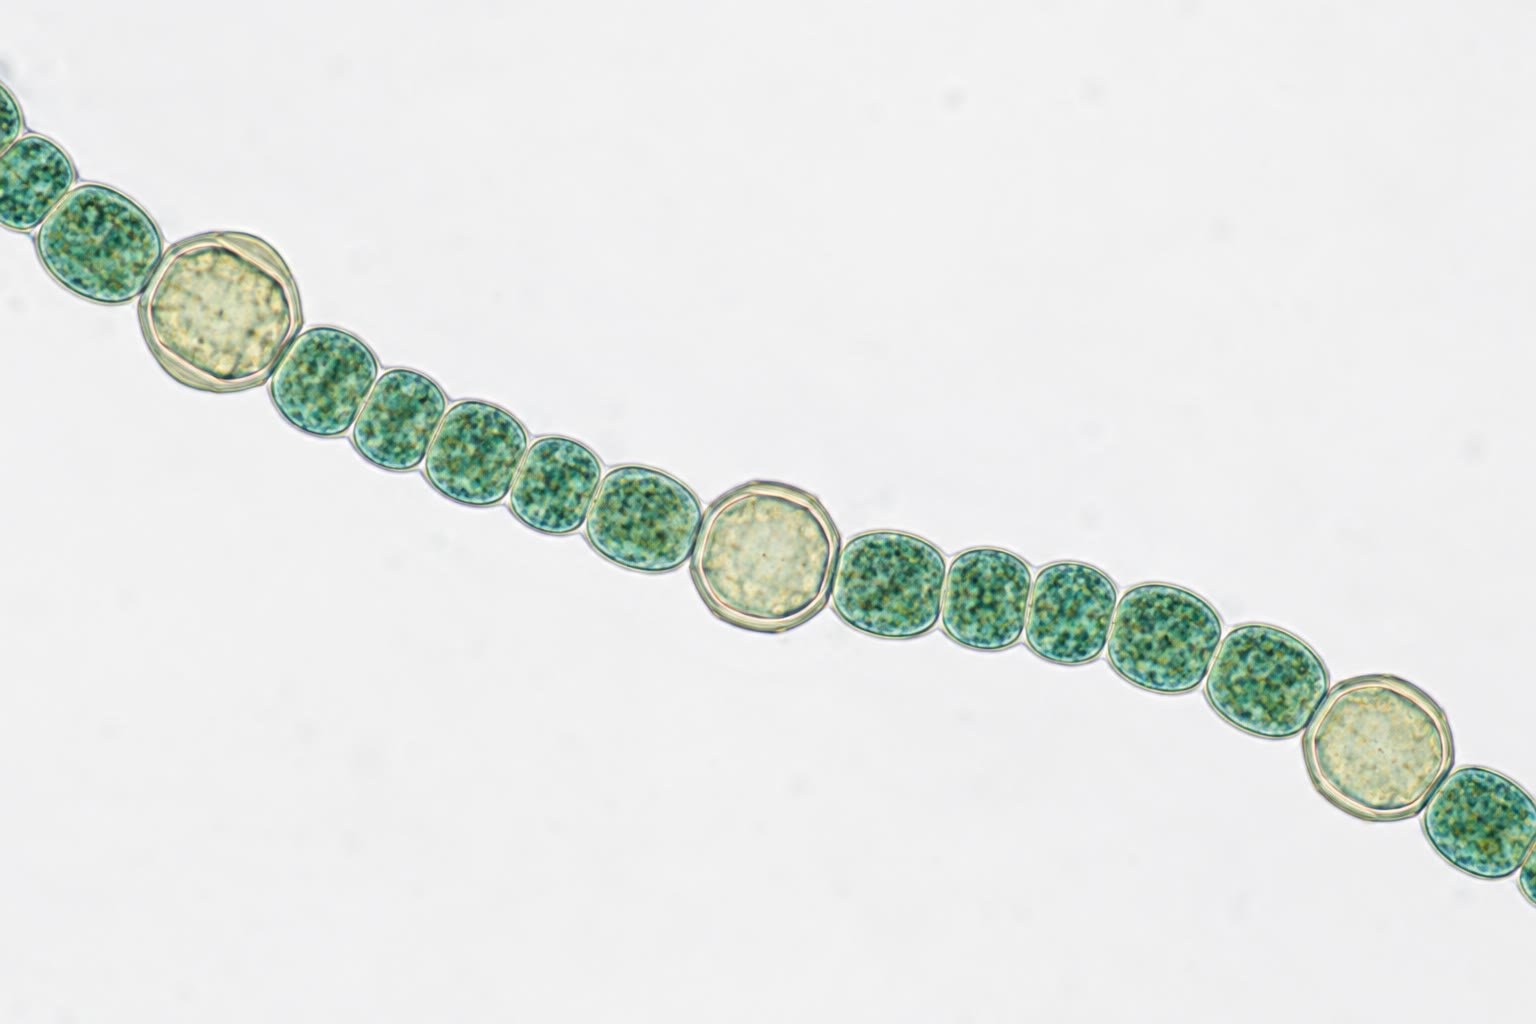
\includegraphics[width=0.62\linewidth]{images/book4/ai/b4-01-anabaena.jpg}

{\small \emph{Anabaena} का एक तंतु: हरी प्रकाशसंश्लेषी कोशिकाओं की एक
शृंखला, जिसे बड़ी, हलके रंग की हेटरोसिस्ट कोशिकाएँ बीच-बीच में तोड़ती
हैं --- वही कोशिकाएँ जो नाइट्रोजन स्थिर करती हैं।}
\end{omfigure}

\begin{remark}[प्रसुप्ति]\label{rem:b2:unicellular-diversity:spores}
कुछ ग्राम-धनी छड़ें (\emph{Bacillus}, \emph{Clostridium}) भुखमरी का उत्तर
\emph{अंतःबीजाणु} बनाकर देती हैं: गुणसूत्र की एक प्रति, कई निर्जलित
आवरणों में लिपटी, उपापचय में निष्क्रिय, खौलने, विकिरण और सदियों के सूखे
की प्रतिरोधी, जो परिस्थितियाँ लौटने पर अंकुरित होती है। अनेक \omterm{def:b2:unicellular-diversity:protist}{प्रोटिस्ट}
यही काम किसी \emph{पुटी} से करते हैं। गतिशीलता के साथ-साथ प्रसुप्ति बुरे
मौसम से बचने का दूसरा रास्ता है।
\end{remark}

\section{एककोशिकीय सुकेंद्रकी जीव}

\begin{definition}[प्रोटिस्ट: एक स्तर, समूह नहीं]\label{def:b2:unicellular-diversity:protist}
\emph{प्रोटिस्ट}\index{प्रोटिस्ट} वे सुकेंद्रकी हैं जो न प्राणी हैं, न
स्थलीय पौधे, न कवक --- अधिकतर \omterm{def:b2:unicellular-diversity:unicellular}{एककोशिकीय}, कुछ \omterm{def:b2:unicellular-diversity:unicellular}{निवही}, थोड़े-से (केल्प)
\omterm{def:b2:unicellular-diversity:unicellular}{बहुकोशिकीय}। उनमें वर्ष 1 के खंड वाली सुकेंद्रकी कोशिका साझी है (केंद्रक,
सूत्रकणिकाएँ, अंतःझिल्लियाँ, कोशिका-कंकाल, $9+2$ पक्ष्माभ) और विशेष रूप
से और कुछ नहीं: जिन वंशक्रमों में वे आते हैं वे एक-दूसरे से उतने ही दूर
हैं जितने प्राणी पौधों से। हरी शैवाल स्थलीय पौधों के साथ हैं; डायटम और
भूरी शैवाल अपना ही एक वंशक्रम बनाते हैं; पक्ष्माभी, डाइनोफ्लैजेलेट और
मलेरिया परजीवी एक और; अमीबा तथा श्लेष्म कवक इन सबसे अधिक प्राणियों और
कवकों के निकट हैं। यह शब्द संगठन के एक स्तर का नाम है --- अकेली जीती
सुकेंद्रकी कोशिका --- न कि वृक्ष की किसी शाखा का।
\end{definition}

\begin{example}[अकेली सुकेंद्रकी कोशिका होने के चार ढंग]\label{ex:b2:unicellular-diversity:four}
\emph{Chlamydomonas}: सेलुलोस-रहित ग्लाइकोप्रोटीन भित्ति, एक प्याले-आकार
का हरितलवक, एक नारंगी नेत्रबिंदु जो किसी प्रकाश-संवेदी पर छाया डालता है
ताकि घूमती हुई कोशिका जान सके कि प्रकाश किधर है, और छाती-तैराकी करते दो
अग्र कशाभ --- ऐसी अंडाकार हरी शैवाल; वह प्रकाशपोषी है।
\emph{Paramecium}: एक पक्ष्माभी, जिसका पूरा पृष्ठ पक्ष्माभों की समन्वित
तरंगों से स्पंदित रहता है, जिसमें मुख जैसी एक मुखीय नाली जीवाणुओं को
भोजन-रसधानियों में बुहारती है, दो संकुचनशील रसधानियाँ हैं, और दो प्रकार
के केंद्रक हैं --- एक छोटा जननिक \emph{लघुकेंद्रक} और एक बड़ा कामकाजी
\emph{गुरुकेंद्रक} जिसमें हर जीन की सैकड़ों प्रतियाँ हैं; वह भक्षपोषी है।
\emph{Amoeba}: न भित्ति, न कोई निश्चित आकार, जो \emph{कूटपादों} से चलता
और खाता है, और उन्हें ऐक्टिन का बहुलकीकरण बाहर धकेलता है। डायटम:
प्रकाशसंश्लेषी कोशिका, जो सिलिका के दो एक पर एक चढ़े कपाटों में बंद है,
मानो डिब्बा और उसका ढक्कन, और छिद्रों से इतनी अलंकृत कि कभी उन कवचों से
सूक्ष्मदर्शी लेंस परखे जाते थे; विभाजित होने पर हर पुत्री एक कपाट रखती है
और एक नया, छोटा, भीतरी कपाट बनाती है।
\end{example}

\begin{omfigure}
\begin{tikzpicture}[every node/.style={font=\scriptsize}]
  % Paramecium outline (slipper)
  \draw[thick, fill=omProp!8] plot[smooth cycle, tension=0.8] coordinates {(0,0) (1.5,0.9) (3.5,1.1) (5.5,0.7) (6.4,0) (5.5,-0.8) (3.5,-1.1) (1.5,-0.9)};
  % cilia
  \foreach \t in {3,9,...,357} {
    \pgfmathsetmacro{\cx}{3.2+3.25*cos(\t)}
    \pgfmathsetmacro{\cy}{1.08*sin(\t)}
    \pgfmathsetmacro{\dx}{3.2+3.55*cos(\t)}
    \pgfmathsetmacro{\dy}{1.32*sin(\t)}
    \draw[gray] (\cx,\cy) -- (\dx,\dy);
  }
  % macronucleus and micronucleus
  \draw[thick, fill=omDef!40] (3.2,0.05) ellipse (0.9 and 0.45);
  \fill[omDef!90!black] (2.4,0.55) circle (0.13);
  % oral groove and gullet
  \draw[thick, omThm] (4.3,-0.95) .. controls (3.6,-0.5) and (3.3,-0.2) .. (3.0,-0.35);
  \fill[omThm!30] (2.9,-0.45) circle (0.16);
  % food vacuoles
  \foreach \p in {(1.4,-0.3),(1.0,0.35),(4.8,0.35)} \draw[thick, omExo!80!black, fill=omExo!30] \p circle (0.17);
  % contractile vacuoles
  \foreach \c in {(1.2,0.0),(5.2,-0.2)} {
    \draw[thick, omDef] \c circle (0.28);
    \foreach \a in {0,60,...,300} \draw[omDef] \c ++(\a:0.28) -- ++(\a:0.22);
  }
  % labels
  \draw (2.4,0.55) -- (2.7,1.6) node[above] {लघुकेंद्रक};
  \draw (3.6,0.3) -- (4.8,1.6) node[above] {गुरुकेंद्रक};
  \draw (1.2,0.28) -- (0.3,1.5) node[above, align=center] {संकुचनशील रसधानी\\(अरीय नलिकाओं सहित)};
  \draw (5.2,-0.48) -- (6.5,-1.5) node[below] {संकुचनशील रसधानी};
  \draw (4.3,-0.95) -- (4.7,-1.75) node[below] {मुखीय नाली};
  \draw (2.9,-0.61) -- (2.7,-1.6) node[below, align=center] {गुहिका और बनती हुई\\भोजन-रसधानी};
  \draw (1.4,-0.47) -- (0.0,-1.5) node[below] {भोजन-रसधानियाँ};
  \draw (6.35,0.4) -- (6.9,1.2) node[above, align=center] {पक्ष्माभ};
\end{tikzpicture}

{\small \emph{Paramecium}, आरेखी: पक्ष्माभित बाह्यक, दोनों केंद्रक, वह
मुखीय नाली जो उस गुहिका तक ले जाती है जहाँ भोजन-रसधानियाँ बनती हैं, और
वे दो तारे जैसी संकुचनशील रसधानियाँ जो परासरण से भीतर आते जल को बाहर
फेंकती हैं।}
\end{omfigure}

\begin{omfigure}
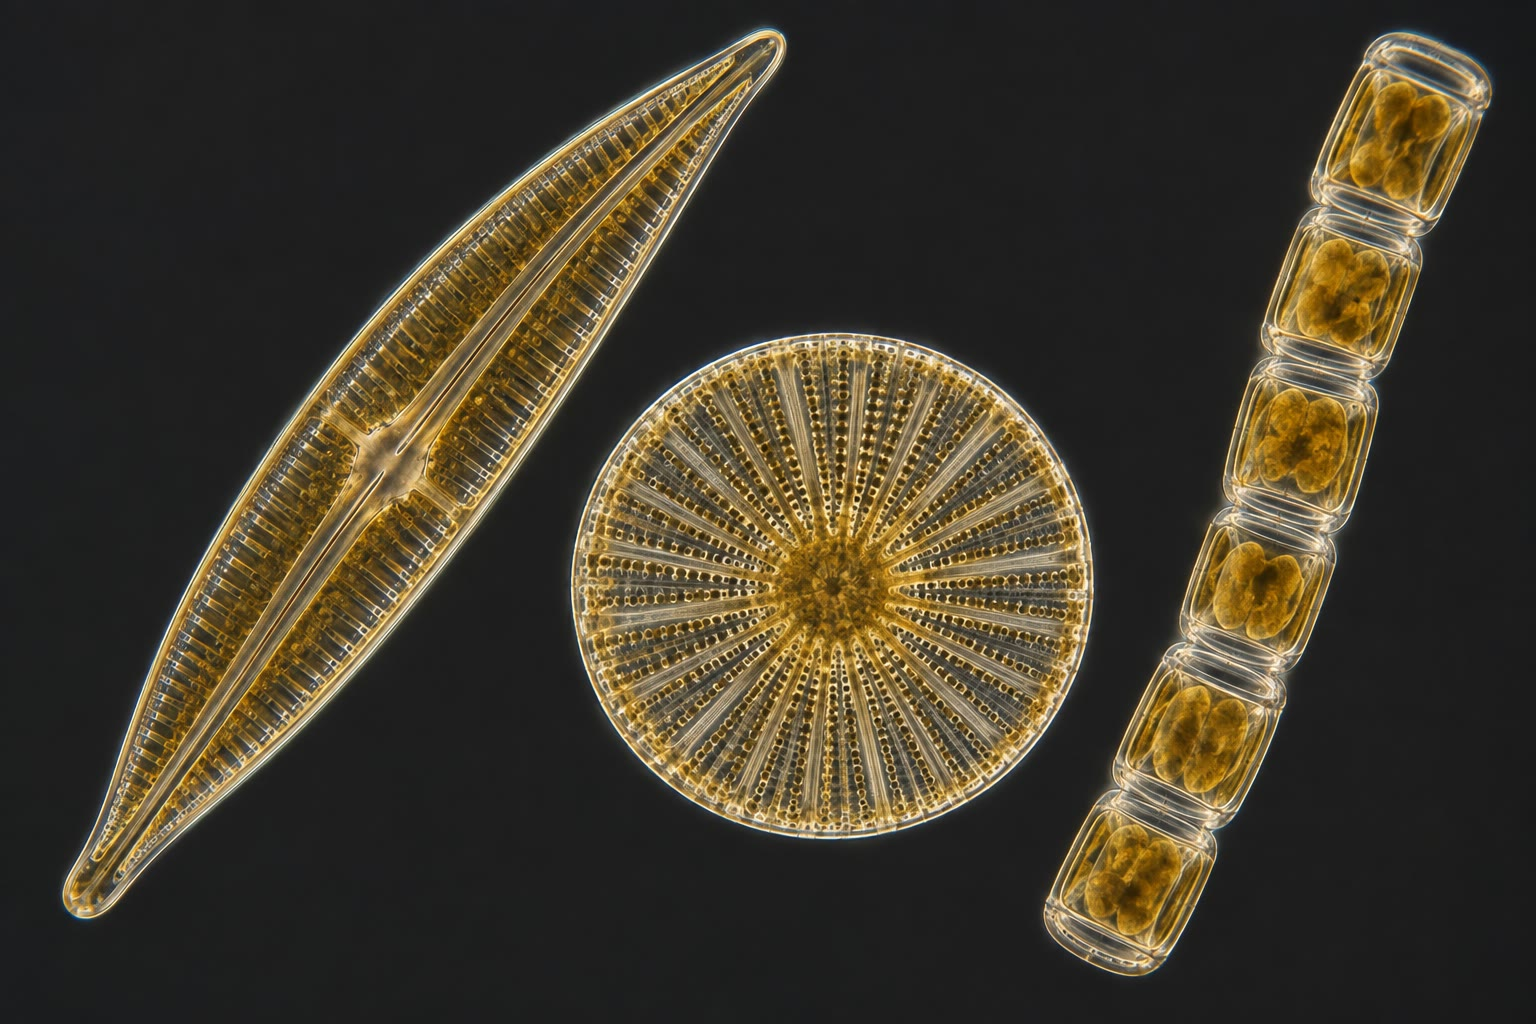
\includegraphics[width=0.6\linewidth]{images/book4/ai/b4-01-diatoms.jpg}

{\small कृष्ण-क्षेत्र सूक्ष्मदर्शन में दिखते डायटम: हर कोशिका सिलिका के
दो-कपाटी कवच में रहती है, जो उन छिद्रों से नक़्क़ाशीदार है जिनसे वह जल
के साथ विनिमय करती है।}
\end{omfigure}

\begin{definition}[पोषण के ढंग]\label{def:b2:unicellular-diversity:nutrition}
\index{भक्षपोषण}\index{परासरणपोषण}\index{मिश्रपोषण}
कोई \omterm{def:b2:unicellular-diversity:unicellular}{एककोशिकीय} सुकेंद्रकी तीन में से एक ढंग से, या एक साथ दो ढंगों से,
पोषण पाता है। \emph{प्रकाशपोषण}: उसके पास हरितलवक हैं और वह प्रकाश तथा
$\mathrm{CO_2}$ से अपना कार्बनिक पदार्थ स्वयं बनाता है (हरी शैवाल,
डायटम, डाइनोफ्लैजेलेट)। \emph{भक्षपोषण}: वह कणों को --- जीवाणुओं को,
दूसरे \omterm{def:b2:unicellular-diversity:protist}{प्रोटिस्टों} को --- किसी भोजन-रसधानी में निगल लेता है, जहाँ लयनकाय
के एंजाइम उन्हें पचा देते हैं (अमीबा, पक्ष्माभी, कॉलरकशाभी)।
\emph{परासरणपोषण}: वह घुले हुए अणुओं को अपनी झिल्ली के आरपार सोखता है,
प्रायः बाहर एंजाइम स्रावित करने के बाद (खमीर, अनेक परजीवी)।
\emph{मिश्रपोषी}, जैसे \emph{Euglena}, उजाले में प्रकाशसंश्लेषण करते हैं
और अँधेरे में खाते हैं। \omterm{def:b2:unicellular-diversity:prokaryote}{प्राक्केंद्रकी} भक्षण नहीं कर सकते: भित्ति मना
करती है, और इसीलिए कोई \omterm{def:b2:unicellular-diversity:prokaryote}{प्राक्केंद्रकी} निगलकर परभक्षी कभी नहीं बना।
\end{definition}

\begin{proposition}[मीठे जल में परासरण-नियमन]\label{prop:b2:unicellular-diversity:osmoregulation}
\index{संकुचनशील रसधानी}
मीठे जल का कोई \omterm{def:b2:unicellular-diversity:protist}{प्रोटिस्ट} भीतर से तालाब की अपेक्षा कहीं अधिक लवणीय है
(कोई \qty{100}{mmol/L} विलेय, तालाब में लगभग \qty{1}{mmol/L}), और उसकी
झिल्ली जल को आने देती है। इसलिए जल परासरण से लगातार भीतर आता है, ऐसी दर
से जो पृष्ठ क्षेत्रफल के और परासरण दाब के अंतर
$\Delta\Pi = RT\,\Delta c$ के समानुपाती है --- ऊपर के आँकड़ों के लिए
लगभग \qty{2.4}{bar}। भित्तिवाली कोशिका स्फीति से टिकी रहती है; नंगी
कोशिका मिनटों में फूलकर फट जाती। \emph{\omterm{prop:b2:unicellular-diversity:osmoregulation}{संकुचनशील रसधानी}} इसका उत्तर है:
एक कुंड, जिसे अरीय नलिकाएँ भरती हैं और जिसमें प्रोटॉन-चालित वाहक जल
पंप करते हैं, और फिर वह सिकुड़कर उस जल को एक छिद्र से बाहर फेंक देता है,
कुछ सेकंड से लेकर कुछ मिनट के अंतराल पर। कोई \emph{Paramecium} हर आधे
घंटे में अपने आयतन जितना जल निकालता है; समुद्री सगे, जो अपने ही जितने
लवणीय माध्यम में रहते हैं, कोई \omterm{prop:b2:unicellular-diversity:osmoregulation}{संकुचनशील रसधानी} रखते ही नहीं।
\end{proposition}

\section{किसी छोटे तैराक की भौतिकी}

\begin{proposition}[निम्न रेनॉल्ड्स संख्या पर जीवन]\label{prop:b2:unicellular-diversity:reynolds}
\index{रेनॉल्ड्स संख्या}
\emph{\omterm{prop:b2:unicellular-diversity:reynolds}{रेनॉल्ड्स संख्या}} $Re = \rho v L/\eta$ किसी $L$ आकार के उस पिंड के
लिए, जो $v$ चाल से $\rho$ घनत्व और $\eta$ श्यानता वाले तरल में चल रहा है,
जड़त्वीय और श्यान बलों की तुलना करती है। मानव तैराक के लिए वह लगभग
$10^6$ है; \emph{Paramecium} (\qty{200}{\micro m},
\qty{1}{mm/s}) के लिए 0.2, और किसी जीवाणु के लिए $10^{-5}$।
$Re \approx 1$ से नीचे जड़त्व बेमानी है: स्पंदन रोकती कोशिका एक
नैनोमीटर के भीतर रुक जाती है, जल गाढ़ी चाशनी जैसा लगता है, और कोई
प्रतिवर्ती गति (आगे और पीछे वही आघात) कोई शुद्ध विस्थापन नहीं देती।
इसलिए छोटे तैराक अप्रतिवर्ती आघात काम में लाते हैं: जीवाणु-कशाभ की घूमती
कुंडली, किसी पक्ष्माभ का असममित स्पंदन (कड़ा शक्ति-आघात, मुड़ा हुआ
वापसी-आघात), \emph{Chlamydomonas} की छाती-तैराकी।
\end{proposition}

\begin{theorem}[स्टोक्स का नियम और डूबना]\label{thm:b2:unicellular-diversity:stokes}
\index{स्टोक्स का नियम}
$r$ त्रिज्या और $\rho_{\text{कोशिका}}$ घनत्व का कोई गोला $\eta$ श्यानता के
तरल में धीरे चले तो उस पर $F = 6\pi\eta r v$ कर्षण लगता है। $\rho$
घनत्व के जल में अपने भरोसे छोड़ दिया जाए तो वह इस सीमांत चाल से डूबता
है:
\[
v_s = \frac{2\,r^2\,(\rho_{\text{कोशिका}} - \rho)\,g}{9\eta},
\]
जो उसकी त्रिज्या के वर्ग के समानुपाती है: दस गुना बड़ी कोशिका सौ गुना
तेज़ डूबती है। इसीलिए पादपप्लवक छोटा है, इसीलिए डायटम काँटे और तेल की
बूँदें ढोते हैं, और इसीलिए तैरना छोड़ देने वाला कोई
\emph{Chlamydomonas} कुछ ही दिनों में प्रकाश से नीचे उतर जाता है।
\end{theorem}
\begin{proof}
सीमांत चाल पर कर्षण आभासी भार (भार घटा उत्प्लावन) को संतुलित करता है:
$6\pi\eta r v_s = \tfrac{4}{3}\pi r^3
(\rho_{\text{कोशिका}} - \rho) g$। $v_s$ के लिए हल करने पर सूत्र मिलता है।
कर्षण का नियम स्वयं भौतिकी की शृंखला में $Re \ll 1$ के लिए व्युत्पन्न
किया गया है; यहाँ उसे दिया हुआ मान लिया गया है।
\end{proof}

\begin{example}[किसी डायटम का गिरना]\label{ex:b2:unicellular-diversity:fall}
\qty{10}{\micro m} त्रिज्या का कोई केंद्रीय डायटम, जो समुद्री जल से
\qty{100}{kg/m^3} अधिक घना है ($\eta = \qty{1e-3}{Pa.s}$), इस चाल से
डूबता है: $v_s = 2\times 10^{-10}\times 100\times 9.81/(9\times 10^{-3}) =
\qty{2.2e-5}{m/s}$, यानी लगभग \qty{2}{m} प्रतिदिन: वह \qty{50}{m} की
प्रकाशित परत महीने भर से भी कम में छोड़ देता। उसकी आबादियाँ इसलिए बची
रहती हैं कि विक्षोभ जल को मथता रहता है, कि तेल की बूँदें और कम घनत्व
$\rho_{\text{कोशिका}} - \rho$ को घटा देते हैं, और कि जो कोशिका डूबते-डूबते
विभाजित हो जाती है वह ऐसी संतति छोड़ती है जो फिर ऊपर उठा दी जाती है।
\end{example}

\begin{omfigure}
\begin{tikzpicture}
\begin{axis}[
  width=0.8\linewidth, height=6.0cm,
  axis x line=bottom, axis y line=left,
  xmode=log, ymode=log,
  xmin=0.5, xmax=200, ymin=1e-3, ymax=1e4,
  xlabel={त्रिज्या (\unit{\micro m})}, ylabel={डूबने की चाल (\unit{\micro m/s})},
  xlabel style={font=\small, at={(axis description cs:0.5,-0.1)}, anchor=north},
  ylabel style={font=\small},
  tick label style={font=\small},
  clip=false,
]
\addplot[very thick, omDef, domain=0.5:200, samples=40] {0.218*x^2};
\addplot[only marks, mark=*, mark size=1.8pt, omThm] coordinates {(1,0.218) (10,21.8) (100,2180)};
\node[font=\scriptsize, anchor=west] at (axis cs:1.15,0.218) {जीवाणु};
\node[font=\scriptsize, anchor=west] at (axis cs:11.5,21.8) {डायटम};
\node[font=\scriptsize, anchor=east] at (axis cs:85,2180) {बड़ा प्रोटिस्ट};
\end{axis}
\end{tikzpicture}

{\small जल से \qty{100}{kg/m^3} अधिक घनी कोशिकाओं के लिए त्रिज्या के
सापेक्ष स्टोक्स डूबन-चाल। लघुगणकीय अक्षों पर 2 का ढाल वही $r^2$ नियम है:
कोई जीवाणु दिन भर में एक सेंटीमीटर डूबता है, कोई बड़ा \omterm{def:b2:unicellular-diversity:protist}{प्रोटिस्ट} घंटे भर
में दो-एक मीटर।}
\end{omfigure}

\section{एक कोशिका में जनन और लैंगिकता}

\begin{definition}[विभाजन के ढंग]\label{def:b2:unicellular-diversity:division}
\index{द्विविभाजन}\index{मुकुलन}\index{बहुविभाजन}
कोई \omterm{def:b2:unicellular-diversity:unicellular}{एककोशिकीय जीव} विभाजित होकर जनन करता है। \emph{द्विविभाजन}: कोशिका
बढ़कर अपने आकार की दुगुनी हो जाती है और दो बराबर पुत्रियों में बँट जाती
है (जीवाणु, \emph{Paramecium}, \emph{Amoeba})।
\emph{मुकुलन}: माता से एक छोटी पुत्री उगकर अलग हो जाती है (खमीर; माता पर
एक निशान रह जाता है और वह कोई बीस बार मुकुल निकाल सकती है)।
\emph{बहुविभाजन}: कोशिका बड़ी हो जाती है, फिर माता की भित्ति के भीतर तेज़ी
से कई बार विभाजित होकर एक साथ 4, 8, 16 या इससे अधिक पुत्रियाँ छोड़ती है
(\emph{Chlamydomonas}, लाल रक्त कोशिका में मलेरिया परजीवी)। अचर
परिस्थितियों में कोशिकाओं की संख्या चरघातांकी रूप से बढ़ती है,
$N(t) = N_0\,2^{t/T}$, जिसमें $T$ वह
\emph{पीढ़ी काल}\index{पीढ़ी काल} है: समृद्ध माध्यम में \emph{E.~coli}
के लिए बीस मिनट, अनेक शैवालों के लिए एक दिन, कुछ पक्ष्माभियों के लिए एक
सप्ताह। (भोजन के फलन के रूप में वृद्धि पर
\cref{ch:b2:microbial-metabolism} में विचार है।)
\end{definition}

\begin{proposition}[जनन बिना सृजन: \emph{Paramecium} में संयुग्मन]\label{prop:b2:unicellular-diversity:conjugation}
\index{संयुग्मन!पक्ष्माभियों में}
पूरक जनन-प्ररूपों के दो \emph{Paramecium} अपने मुखीय पृष्ठों से जुड़ जाते
हैं। हर एक में द्विगुणित लघुकेंद्रक अर्धसूत्री विभाजन से चार अगुणित
केंद्रक बनाता है, जिनमें से तीन क्षीण हो जाते हैं; बचा हुआ समसूत्री
विभाजन से एक स्थिर और एक प्रवासी केंद्रक में बँटता है, और दोनों कोशिकाएँ
संधि के आरपार अपने प्रवासी केंद्रकों की अदला-बदली कर लेती हैं। फिर हर
कोशिका अपने स्थिर केंद्रक को मिले हुए केंद्रक से मिला देती है, और दोनों
साथी अलग हो जाते हैं, हर एक अपने साथी के ही जीन-प्ररूप का नया द्विगुणित
लघुकेंद्रक लिए। पुराना गुरुकेंद्रक टूट जाता है और नए लघुकेंद्रक से नया
बनाया जाता है। कोई नई कोशिका नहीं बनी: संयुग्मन गुणन से अलग किया गया
आनुवंशिक मिश्रण है --- अर्धसूत्री विभाजन और निषेचन,
\cref{ch:b2:meiosis-heredity}।
जीवाणु-संयुग्मन, जो किसी \omterm{def:b2:unicellular-diversity:prokaryote}{प्लास्मिड} को दाता से ग्राही तक एक ही दिशा में
पहुँचाता है, उसी नाम की एक भिन्न प्रक्रिया है
(\cref{ch:b2:genome-diversification})।
\end{proposition}

\begin{omfigure}
\begin{tikzpicture}[every node/.style={font=\scriptsize}]
  \foreach \i/\x in {0/0,1/3.6,2/7.2,3/10.8} {
    \draw[thick, fill=omProp!8] (\x,0.55) ellipse (1.0 and 0.5);
    \draw[thick, fill=omProp!8] (\x,-0.55) ellipse (1.0 and 0.5);
  }
  % stage 0: two cells, diploid micronuclei 2n
  \fill[omDef!90!black] (0,0.55) circle (0.12); \node[right] at (0.15,0.55) {$2n$};
  \fill[omDef!90!black] (0,-0.55) circle (0.12); \node[right] at (0.15,-0.55) {$2n$};
  \node[below, align=center] at (0,-1.15) {दो कोशिकाएँ जुड़ती हैं};
  % stage 1: meiosis, 4 haploid, 3 degenerate
  \foreach \dy in {0.55,-0.55} {
    \fill[omDef!90!black] (3.6-0.3,\dy+0.15) circle (0.08);
    \fill[gray!60] (3.6+0.1,\dy+0.2) circle (0.06);
    \fill[gray!60] (3.6+0.3,\dy-0.05) circle (0.06);
    \fill[gray!60] (3.6-0.1,\dy-0.25) circle (0.06);
  }
  \node[below, align=center] at (3.6,-1.15) {अर्धसूत्री विभाजन:\\4 अगुणित केंद्रक,\\तीन क्षीण};
  % stage 2: mitosis, exchange
  \foreach \dy in {0.55,-0.55} {
    \fill[omDef!90!black] (7.2-0.35,\dy) circle (0.08);
    \fill[omThm] (7.2+0.35,\dy) circle (0.08);
  }
  \draw[->, thick, omThm] (7.55,0.45) -- (7.55,-0.45);
  \draw[->, thick, omThm] (6.85,-0.45) -- (6.85,0.45);
  \node[below, align=center] at (7.2,-1.15) {समसूत्री विभाजन; प्रवासी\\केंद्रक (लाल)\\बदले जाते हैं};
  % stage 3: fusion 2n
  \fill[omDef!90!black] (10.8,0.55) circle (0.12); \node[right] at (10.95,0.55) {$2n$};
  \fill[omDef!90!black] (10.8,-0.55) circle (0.12); \node[right] at (10.95,-0.55) {$2n$};
  \node[below, align=center] at (10.8,-1.15) {निषेचन:\\नए एक जैसे द्विगुणित\\केंद्रक; कोशिकाएँ अलग};
  \foreach \x in {1.3,4.9,8.5} \draw[->, thick, gray] (\x,0) -- (\x+1.0,0);
\end{tikzpicture}

{\small \emph{Paramecium} में संयुग्मन। दो कोशिकाएँ अगुणित केंद्रकों की
अदला-बदली करके अलग हो जाती हैं, हर एक पुनर्संयोजित द्विगुणित लघुकेंद्रक
लिए; कोशिकाओं की संख्या नहीं बदली।}
\end{omfigure}

\section{बहुकोशिकीयता की ओर}

\begin{proposition}[वॉल्वोसी शृंखला]\label{prop:b2:unicellular-diversity:volvox}
\index{Volvox@\emph{Volvox}}\index{बहुकोशिकीयता की उत्पत्ति}
हरी शैवालों में एक वंशक्रम, जीवित जातियों में ही, एक कोशिका से शरीर तक के
पग दिखा देता है। \emph{Chlamydomonas} अकेली रहती है।
\emph{Gonium} 4 से 16 एक जैसी कोशिकाओं की एक चपटी पट्टिका है जो साथ-साथ
तैरती हैं। \emph{Pandorina} और \emph{Eudorina} 16 से 32 कोशिकाओं की खोखली
गेंदें हैं, अब भी सब एक जैसी, और हर एक नया निवह बसाने में समर्थ।
\emph{Pleodorina} में कुछ छोटी कोशिकाएँ हैं जो केवल तैरती हैं, विभाजित
कभी नहीं होतीं। \emph{Volvox} \num{500} से \num{50000} छोटी कायिक
कोशिकाओं का गोला है, कशाभयुक्त, जो निवह के साथ ही मर जाएँगी, और उनके बीच
मुट्ठी भर बड़ी जनन कोशिकाएँ (गोनिडिया) हैं जो विभाजित होकर माता के भीतर
ही पुत्री-गोले बनाती हैं। कायिक और जननिक कोशिकाएँ प्रकट हो चुकी हैं: यह
बहुकोशिकीयता की देहरी है, जिसे इस वंशक्रम ने कोई \num{200} लाख वर्ष पहले
पार किया और, स्वतंत्र रूप से, जीवन-वृक्ष में और कहीं कम से कम पच्चीस बार
--- प्राणियों, पौधों, कवकों, भूरी शैवालों, लाल शैवालों और जीवाणुओं के कई
समूहों में।
\end{proposition}
\begin{proof}[प्रमाण-सामग्री]
दर्जनों जीनों से बना वॉल्वोसी शैवालों का आणविक जातिवृत्त
\emph{Chlamydomonas} को आधार पर और \emph{Volvox} को सिरों पर रखता है,
बीच में \omterm{def:b2:unicellular-diversity:unicellular}{निवही} रूपों के साथ और शाखाओं के साथ बढ़ती कोशिका-संख्या के साथ;
\emph{Volvox carteri} का जीनोम (2010) \emph{Chlamydomonas} के जीनोम से
कुछ सौ जीनों भर से भिन्न है, मुख्यतः उन जीनों से जो कोशिकाओं को थामे
रखने वाली बाह्यकोशिकीय आधात्री के हैं और उन नियामकों के जो कायिक
कोशिकाओं में विभाजन चुप करा देते हैं। इस संक्रमण को उल्लेखनीय रूप से
थोड़ी ही नई आनुवंशिक सामग्री चाहिए थी।
\end{proof}

\begin{omfigure}
\begin{tikzpicture}[every node/.style={font=\scriptsize}]
  % Chlamydomonas
  \draw[thick, fill=omProp!25] (0,0) circle (0.22);
  \node[below=0.35cm, align=center] at (0,0) {\emph{Chlamydomonas}\\1 कोशिका};
  % Gonium plate
  \begin{scope}[xshift=2.2cm]
    \foreach \x in {-0.3,0,0.3} \foreach \y in {-0.3,0,0.3} \draw[thick, fill=omProp!25] (\x,\y) circle (0.14);
    \draw[gray, dashed] (-0.55,-0.55) rectangle (0.55,0.55);
    \node[below=0.7cm, align=center] at (0,0) {\emph{Gonium}\\8--16 की पट्टिका};
  \end{scope}
  % Eudorina ball
  \begin{scope}[xshift=4.5cm]
    \draw[gray, dashed] (0,0) circle (0.6);
    \foreach \a in {0,45,...,315} \draw[thick, fill=omProp!25] (\a:0.55) circle (0.13);
    \draw[thick, fill=omProp!25] (0,0.1) circle (0.13);
    \node[below=0.7cm, align=center] at (0,0) {\emph{Eudorina}\\32 की गेंद,\\सब एक जैसी};
  \end{scope}
  % Pleodorina
  \begin{scope}[xshift=7.4cm]
    \draw[gray, dashed] (0,0) circle (0.7);
    \foreach \a in {0,30,...,330} \draw[thick, fill=omProp!25] (\a:0.62) circle (0.09);
    \foreach \a in {60,180,300} \draw[thick, fill=omProp!60] (\a:0.62) circle (0.14);
    \node[below=0.8cm, align=center] at (0,0) {\emph{Pleodorina}\\कुछ कोशिकाएँ\\केवल तैरती हैं};
  \end{scope}
  % Volvox
  \begin{scope}[xshift=10.6cm]
    \draw[thick, fill=omProp!6] (0,0) circle (0.95);
    \foreach \a in {0,12,...,348} \fill[omProp!70] (\a:0.9) circle (0.035);
    \foreach \a in {0,12,...,348} \fill[omProp!50] (\a:0.72) circle (0.03);
    \foreach \p in {(0.25,0.2),(-0.3,-0.25),(0.1,-0.4),(-0.2,0.35)} \draw[thick, omThm, fill=omThm!40] \p circle (0.13);
    \node[below=1.05cm, align=center] at (0,0) {\emph{Volvox}\\हज़ारों कायिक कोशिकाएँ\\और कुछ जनन कोशिकाएँ (लाल)};
  \end{scope}
  \foreach \x in {0.5,3.0,5.3,8.3} \draw[->, gray] (\x,0) -- (\x+0.6,0);
\end{tikzpicture}

{\small वॉल्वोसी शृंखला: एक अकेली कोशिका, एक पट्टिका, एक जैसी कोशिकाओं
की खोखली गेंद, एक ऐसी गेंद जिसमें कुछ कोशिकाओं ने विभाजन छोड़ दिया है,
और \emph{Volvox}, जहाँ हज़ारों नश्वर कायिक कोशिकाएँ कुछ जनन कोशिकाओं को
घेरे हैं।}
\end{omfigure}

\begin{omfigure}
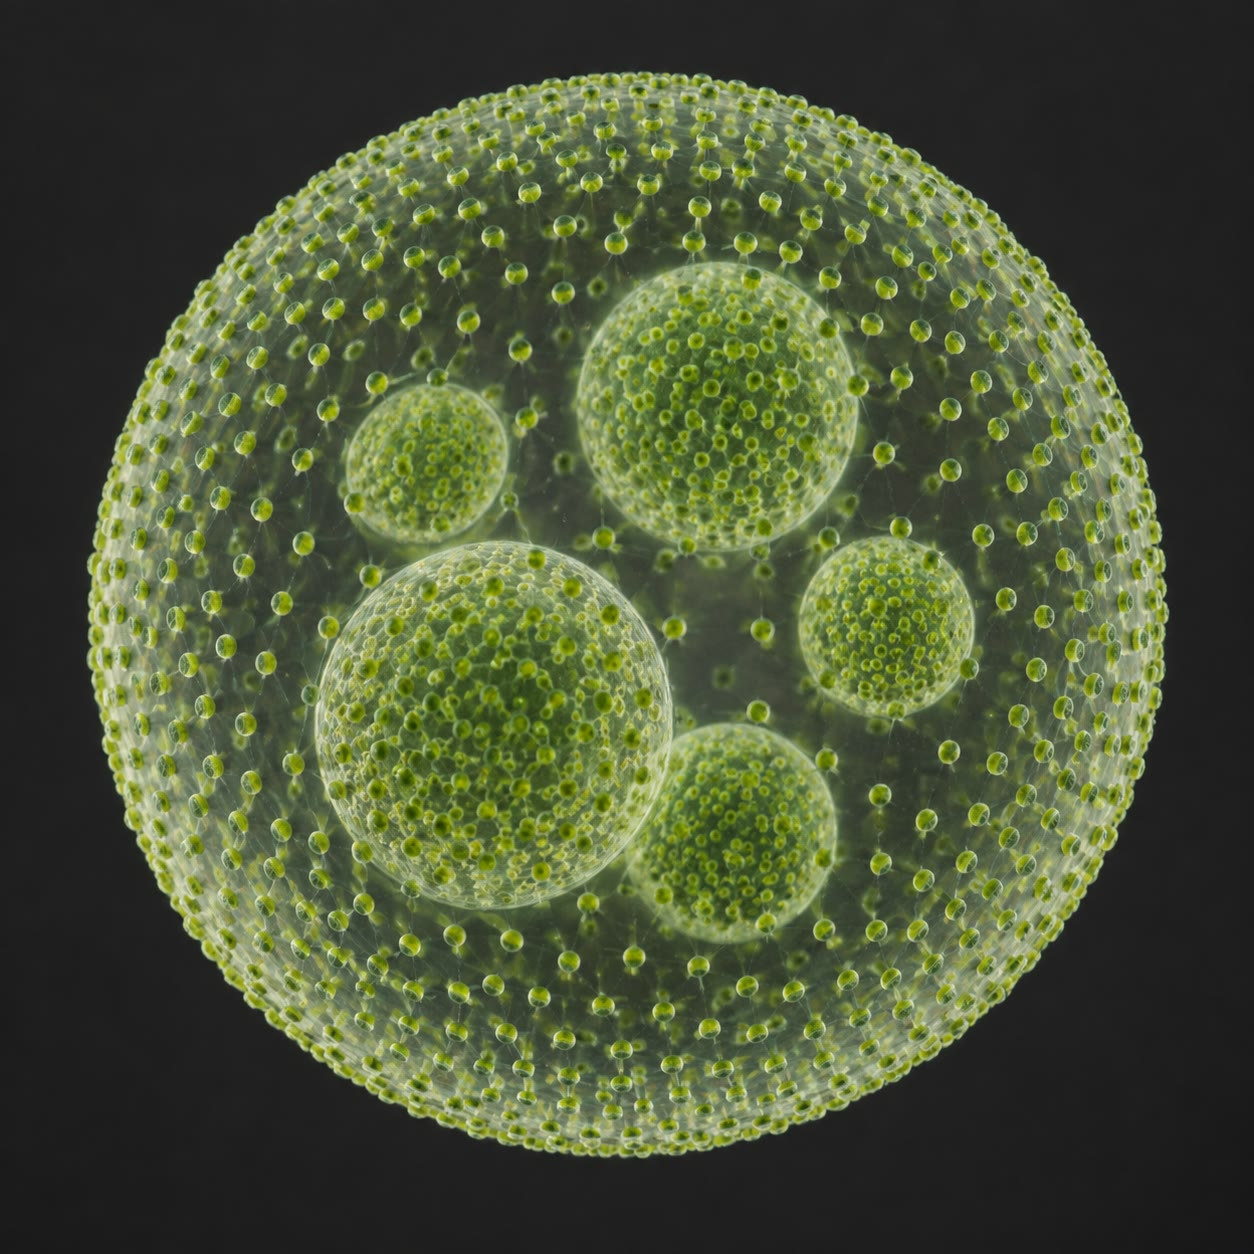
\includegraphics[width=0.55\linewidth]{images/book4/ai/b4-01-volvox.jpg}

{\small \emph{Volvox} का एक निवह: कशाभयुक्त कोशिकाओं का खोखला हरा गोला,
जिसके भीतर पुत्री-निवह उग रहे हैं।}
\end{omfigure}

\begin{remark}[श्रम क्यों बाँटें?]\label{rem:b2:unicellular-diversity:whydivide}
इन शैवालों में कोई कोशिका एक ही समय तैर और विभाजित नहीं हो सकती: कशाभों
को टिकाने वाले आधारकाय तर्कु सजाने के लिए चाहिए। अकेली कोशिका बारी-बारी
से काम लेती है; छोटा निवह इतना सह सकता है कि उसकी सारी कोशिकाएँ विभाजित
होने तक तैरना रुक जाए; बड़ा निवह विभाजन में लगने वाले घंटों में प्रकाश से
नीचे उतर जाता (\omterm{thm:b2:unicellular-diversity:stokes}{स्टोक्स का नियम}, \cref{thm:b2:unicellular-diversity:stokes})।
किसी आकार के आगे कुछ कोशिकाओं को तैरता रखना जबकि दूसरी विभाजित हों,
उनकी संतति के नुक़सान से अधिक मूल्यवान है --- और एक काया जन्म लेती है।
कॉलरकशाभी, यानी वे कॉलरदार कशाभी जिनकी कोशिका स्पंज की भोजन-कोशिका की
प्रतिलिपि है, उसी शाखा पर वही पहले पग दिखाते हैं जो प्राणियों तक ले गई।
\end{remark}

\section{अभ्यास}

\begin{exercise}[$\star$]\label{exo:b2:unicellular-diversity:1}
\omterm{def:b2:unicellular-diversity:unicellular}{एककोशिकीय}, \omterm{def:b2:unicellular-diversity:unicellular}{निवही} और \omterm{def:b2:unicellular-diversity:unicellular}{बहुकोशिकीय} की परिभाषा दीजिए, और
\emph{E.~coli}, \emph{Gonium}, \emph{Volvox} तथा खमीर की कोशिका को
कारण सहित सही वर्ग में रखिए।
\end{exercise}

\begin{exercise}[$\star$]\label{exo:b2:unicellular-diversity:2}
\qty{0.5}{\micro m} त्रिज्या के किसी गोलाणु का और \qty{50}{\micro m}
त्रिज्या के किसी गोलीय \omterm{def:b2:unicellular-diversity:protist}{प्रोटिस्ट} का \omterm{prop:b2:unicellular-diversity:surface}{पृष्ठ-आयतन अनुपात} निकालिए। प्रति
इकाई कोशिकाद्रव्य कौन तेज़ी से श्वसन करता है, और क्यों?
\end{exercise}

\begin{exercise}[$\star$]\label{exo:b2:unicellular-diversity:3}
किसी जीवाणु और किसी \omterm{def:b2:unicellular-diversity:unicellular}{एककोशिकीय} सुकेंद्रकी के बीच तीन संरचनात्मक भेद
बताइए, और एक ऐसी बात जो कोई जीवाणु नहीं कर सकता पर कोई अमीबा कर सकता है।
\end{exercise}

\begin{exercise}[$\star$]\label{exo:b2:unicellular-diversity:4}
\emph{Paramecium} की इन संरचनाओं में से हर एक का कार्य बताइए: पक्ष्माभ,
मुखीय नाली, भोजन-रसधानी, \omterm{prop:b2:unicellular-diversity:osmoregulation}{संकुचनशील रसधानी}, गुरुकेंद्रक, लघुकेंद्रक।
\end{exercise}

\begin{exercise}[$\star\star$]\label{exo:b2:unicellular-diversity:5}
कोशिकाद्रव्य में किसी उपापचयज के लिए $D = \qty{5e-10}{m^2/s}$ लेने पर,
\qty{1}{\micro m} के जीवाणु के आरपार और \qty{500}{\micro m} के अमीबा के
आरपार विसरण में कितना समय लगता है? अमीबा को जो करना ही पड़ता है और
जीवाणु को नहीं, उस पर टिप्पणी कीजिए।
\end{exercise}

\begin{exercise}[$\star\star$]\label{exo:b2:unicellular-diversity:6}
किसी \emph{Paramecium} (\qty{200}{\micro
m}, \qty{1}{mm/s}), किसी जीवाणु (\qty{2}{\micro m}, \qty{20}{\micro
m/s}) और किसी मानव तैराक (\qty{2}{m}, \qty{1}{m/s}) की \omterm{prop:b2:unicellular-diversity:reynolds}{रेनॉल्ड्स संख्या}
$\rho = \qty{1000}{kg/m^3}$ और $\eta = \qty{1e-3}{Pa.s}$ के साथ
निकालिए। कोई तैराक एक आघात के बाद फिसलता क्यों चला जाता है और कोई जीवाणु
नहीं?
\end{exercise}

\begin{exercise}[$\star\star$]\label{exo:b2:unicellular-diversity:7}
\qty{10}{\micro m} त्रिज्या का कोई डायटम जल से \qty{100}{kg/m^3} अधिक
घना है। उसकी डूबन-चाल और \qty{50}{m} गिरने में लगने वाला काल निकालिए।
कोशिका अपनी त्रिज्या आधी कर ले तो यह काल कितने गुना बदलता है? और अपना
अतिरिक्त घनत्व घटाकर \qty{20}{kg/m^3} कर ले तो?
\end{exercise}

\begin{exercise}[$\star\star$]\label{exo:b2:unicellular-diversity:8}
किसी \emph{Paramecium} को \num{100}, \num{25} और \qty{25}{\micro m}
अर्ध-अक्षों के दीर्घवृत्ताभ के रूप में लीजिए ($V = \tfrac{4}{3}\pi abc$)।
वह हर \qty{30}{min} में अपने आयतन जितना जल बाहर फेंकता है। जल का अंतर्वाह
\unit{\micro m^3/s} में और लिटर प्रति सेकंड में निकालिए।
\end{exercise}

\begin{exercise}[$\star\star$]\label{exo:b2:unicellular-diversity:9}
कोई आकर्षी \qty{1}{mm} में अपनी सांद्रता दुगुनी कर लेता है।
\qty{1}{\micro m} के किसी जीवाणु के दोनों सिरों के बीच सापेक्ष अंतर कितना
है? \qty{20}{\micro m/s} पर \qty{1}{s} की दौड़ के आरंभ और अंत के बीच
कितना? $N$ अणु गिनने में लगभग $1/\sqrt{N}$ की सापेक्ष त्रुटि होती है:
समझाइए कि जीवाणु पक्षों की नहीं बल्कि समयों की तुलना क्यों करता है।
\end{exercise}

\begin{exercise}[$\star\star\star$]\label{exo:b2:unicellular-diversity:10}
\emph{Thiomargarita namibiensis} \qty{500}{\micro m} व्यास का एक गोलीय
गंधक-जीवाणु है, जिसका कोशिकाद्रव्य नाइट्रेट की एक रसधानी के चारों ओर
\qty{2}{\micro m} मोटा खोल है। उसके पृष्ठ का उसके \emph{कोशिकाद्रव्यी}
आयतन से अनुपात निकालिए और \emph{E.~coli} से तुलना कीजिए
(\qty{0.5}{\micro m} त्रिज्या का बेलन; सिरे छोड़ दीजिए)। समझाइए कि वह
रसधानी उसे इतना बड़ा होने कैसे देती है, और नाइट्रेट किस काम आता है।
\end{exercise}

\begin{exercise}[$\star\star\star$]\label{exo:b2:unicellular-diversity:11}
\emph{Volvox} में कायिक कोशिकाएँ कभी विभाजित नहीं होतीं और निवह के साथ
मर जाती हैं। कशाभन की बाध्यता और \omterm{thm:b2:unicellular-diversity:stokes}{स्टोक्स का नियम} काम में लेकर समझाइए कि
ऐसी कोशिकाएँ \num{10000} कोशिकाओं के निवह में रखने योग्य क्यों हैं पर
16 के निवह में नहीं, और जनन कोशिकाएँ गोले की सबसे बड़ी कोशिकाएँ क्यों
हैं।
\end{exercise}

\begin{exercise}[$\star\star\star$]\label{exo:b2:unicellular-diversity:12}
``\omterm{def:b2:unicellular-diversity:protist}{प्रोटिस्ट} एक स्तर है, क्लेड नहीं।'' इस अध्याय में नामित वंशक्रमों से
यह भेद समझाइए, और बताइए कि वही कथन ``\omterm{def:b2:unicellular-diversity:prokaryote}{प्राक्केंद्रकी}'' के लिए सच और
``सायनोजीवाणु'' के लिए झूठ क्यों है।
\end{exercise}

\section{समस्या: तालाब के पानी की एक बूँद}

\begin{problem}[{सप्तांत समस्या --- तालाब के पानी का एक प्रतिदर्श गिना
जाता है, उगाया जाता है, और उसकी कोशिकाओं को चलाने वाली भौतिकी के लिए
विश्लेषित किया जाता है, और अंत किसी हरी शैवाल के जल तथा ऊर्जा बजट पर}]
\label{pb:b2:unicellular-diversity:1}
वसंत में \qty{1000}{m^3} के किसी तालाब का प्रतिदर्श लिया जाता है।
सूक्ष्मदर्शी के नीचे, एक गणन-कक्ष, जिसकी जाली \qty{1}{mm}$\times$\qty{1}{mm}
घेरती है और जिसके ऊपर \qty{0.1}{mm} पर एक आवरण-पट्टी टिकी है, उसमें
\emph{Chlamydomonas} की 24 कोशिकाएँ दिखती हैं (\qty{5}{\micro m}
त्रिज्या के गोले, घनत्व \qty{1050}{kg/m^3})। $\rho = \qty{1000}{kg/m^3}$,
$\eta = \qty{1e-3}{Pa.s}$, $g = \qty{9.81}{m/s^2}$, $R =
\qty{8.314}{J/mol/K}$, $T = \qty{293}{K}$, और $D = \qty{1.9e-9}{m^2/s}$
(जल में $\mathrm{CO_2}$ के लिए) लीजिए।

\medskip
\noindent\textbf{भाग I --- गिनती।}
\begin{enumerate}
  \item जाली के नीचे के जल का आयतन माइक्रोलिटर में निकालिए।
  \item इससे तालाब में \emph{Chlamydomonas} का घनत्व, कोशिकाएँ प्रति
        मिलिलिटर में, निकालिए।
  \item एक कोशिका का आयतन और उसका \omterm{prop:b2:unicellular-diversity:surface}{पृष्ठ-आयतन अनुपात} निकालिए।
  \item तालाब के जल के आयतन का कितना अंश इन कोशिकाओं ने घेरा है?
  \item तालाब में कितने \emph{Chlamydomonas} हैं?
  \item एक तंतुमय सायनोजीवाणु भी उपस्थित है। सूक्ष्मदर्शी के नीचे दिखने
        वाले दो ऐसे लक्षण बताइए जो उसे शैवाल से अलग करते हैं।
\end{enumerate}

\medskip
\noindent\textbf{भाग II --- वृद्धि।}
प्रतिदर्श प्रकाश में रखा जाता है और \qty{48}{h} बाद फिर गिना जाता है:
जाली के नीचे \num{384} कोशिकाएँ।
\begin{enumerate}[resume]
  \item \omterm{def:b2:unicellular-diversity:division}{पीढ़ी काल} $T$ निकालिए।
  \item वृद्धि दर स्थिरांक $k$ को $N = N_0 e^{kt}$ में, \unit{h^{-1}} की
        इकाई में, निकालिए।
  \item इसी दर पर तालाब की आबादी को \qty{1e8}{} कोशिकाएँ प्रति मिलिलिटर
        तक पहुँचने में कितना समय लगता?
  \item तीन कारण बताइए कि वह नहीं पहुँचेगी।
  \item यदि कोशिकाएँ केवल \qty{12}{h} के दिन-उजाले में बढ़ें और रात में
        बिलकुल नहीं, तो वही वृद्धि कितने समय में होती है?
  \item \emph{Chlamydomonas} \omterm{def:b2:unicellular-diversity:division}{बहुविभाजन} से विभाजित होती है और एक साथ
        4, 8 या 16 पुत्रियाँ छोड़ती है। समझाइए कि फिर भी गिनती से \omterm{def:b2:unicellular-diversity:division}{पीढ़ी
        काल} भली-भाँति परिभाषित क्यों है।
\end{enumerate}

\medskip
\noindent\textbf{भाग III --- कोशिका की भौतिकी।}
\begin{enumerate}[resume]
  \item \qty{100}{\micro m/s} पर तैरती किसी कोशिका की \omterm{prop:b2:unicellular-diversity:reynolds}{रेनॉल्ड्स संख्या}
        निकालिए।
  \item $m$ द्रव्यमान की कोई कोशिका अपने कशाभ चलाना बंद कर दे तो
        $mv/(6\pi\eta r)$ दूरी तक बहती चली जाती है। उसे निकालिए।
  \item तैरना बंद कर चुकी किसी कोशिका की डूबन-चाल निकालिए।
  \item \qty{1}{m} डूबने में लगने वाले काल की तुलना \qty{1}{m} ऊपर
        तैरने में लगने वाले काल से कीजिए।
  \item तालाब में \qty{10}{\micro mol/L} घुली हुई
        $\mathrm{CO_2}$ है। किसी कोशिका को $\mathrm{CO_2}$ की अधिकतम
        विसरण-आपूर्ति, अणु प्रति सेकंड में, निकालिए।
  \item किसी कोशिका में \qty{100}{pg} कार्बन है और वह उसे एक पीढ़ी में
        दुगुना कर लेती है। उसकी माध्य कार्बन-माँग अणु प्रति सेकंड में,
        और आपूर्ति का माँग से अनुपात, निकालिए।
  \item उसी कार्बन-घनत्व वाली \qty{50}{\micro m} त्रिज्या की किसी
        काल्पनिक कोशिका के लिए यह तुलना दोहराइए। निष्कर्ष निकालिए।
\end{enumerate}

\medskip
\noindent\textbf{भाग IV --- जल और ऊर्जा।}
कोशिकाद्रव्य में \qty{100}{mmol/L} विलेय हैं, तालाब में
\qty{1}{mmol/L}। झिल्ली की जलचालकता $L_p =
\qty{1e-14}{m.s^{-1}.Pa^{-1}}$ है (प्रति इकाई क्षेत्रफल प्रति इकाई दाब-अंतर
जल का आयतन-अभिवाह)। एक ATP के जल-अपघटन से \qty{50}{kJ/mol} मिलते हैं;
एक कार्बन परमाणु स्थिर करने में तीन ATP लगते हैं।
\begin{enumerate}[resume]
  \item झिल्ली के आरपार परासरण दाब का अंतर निकालिए।
  \item प्रति सेकंड कोशिका में घुसने वाले जल का आयतन
        \unit{\micro m^3/s} में निकालिए।
  \item \omterm{prop:b2:unicellular-diversity:osmoregulation}{संकुचनशील रसधानी} के बिना कोशिका को अपना आयतन दुगुना करने में
        कितना समय लगता?
  \item इस जल को परासरण दाब के विरुद्ध बाहर फेंकने के लिए आवश्यक
        न्यूनतम शक्ति निकालिए।
  \item उसे ATP अणु प्रति सेकंड में बदलिए और कार्बन-स्थिरीकरण पर कोशिका
        के ख़र्च होते ATP से तुलना कीजिए (प्रश्न 18)।
  \item परिणाम बताइए: कोशिका में जल का अंतर्वाह, उसे फटने में लगने वाला
        काल, और सूखा रहने में उसकी ऊर्जा का कितना अंश ख़र्च होता है।
\end{enumerate}
\end{problem}
